\newpage
\section{Teilversuch 2: Bewegungsvorgang eines Maxwellschen Rads}
    \subsection{Messung mittels Spiegelskala und Stoppuhr}
        Aufgrund der Art der Schwingung des Maxwellschen Rads können wir den Umkehrpunkt erst nach der Umkehrung bestimmen. Das hat bei dieser Messung zu einem Messfehler geführt, der größer als die menschliche Reaktionszeit von $\SI{0.2}{\second}$ ist. In diesem Fall war $\Delta T = \SI{0,5}{\milli\meter}$ geschätzt. 

        Fehler beim Ablesen der Spiegelskala $= \SI{5}{\milli\meter}$\\
        Fehler bei Messung mittels Stoppuhr\footnote{Im Protokoll war der Fehler als $\pm \SI{1}{\second}$ geschätzt. Das fanden wir rückblickend zu groß eine Überschätzung.} $= \SI{0,5}{\second}$

        \textbf{Messreihen:}
        \begin{center}
            \begin{tabular}{l *{11}{r}}
                \toprule
                $n$ & $1$ & $2$ & $3$ & $4$ & $5$ & $6$ & $7$ & $8$ & $9$ & $10$ & $11$ \\
                \midrule
                Höhe $h_n$ / \SI{}{\milli\meter} & $775$ & $715$ & $665$ & $647$ & $583$ & $550$ & $515$ & $485$ & $465$ & $430$ & $405$ \\
                Periode $T_n$ / \SI{}{\second} & $10,57$ & $9,53$ & $10,10$ & $8,92$ & $8,89$ & $8,76$ & $7,79$ & $7,59$  & $7,92$ & $7,40$ & $7,03$  \\
                $T_n^2$ / \SI{}{\second\squared} & $111,7$ & $90,8$ & $102,0$ & $79,6$ & $79,0$ & $76,7$ & $60,7$ & $57,6$ & $62,7$ & $54,8$ & $49,4$ \\
                \bottomrule
                \toprule
                $n$ & $12$ & $13$ & $14$ & $15$ & $16$ & $17$ & $18$ & $19$ & $20$ & $21$ &  \\
                \midrule
                Höhe $h_n$ / \SI{}{\milli\meter} & $387$ & $365$ & $345$ & $330$ & $315$ & $300$ & $296$ & $275$ & $260$ & $250$  & \\
                Periode $T_n$ / \SI{}{\second} & $6,52$ & $6,41$ & $6,55$ & $5,64$ & $6,07$ & $5,30$ & $5,48$ & $5,04$ & $4,69$ & $4,76$ &  \\
                $T_n^2$ / \SI{}{\second\squared} & $42,5$ & $41,1$ & $42,9$ & $31,8$ & $36,8$ & $28,1$ & $30,0$ & $25,4$ & $22,0$ & $22,7$ & \\
                \bottomrule
            \end{tabular}
        \end{center}
        wobei $n$ die Schwingungsnummer ist. 

        Der erste Höhenwert im Protokoll entspricht der Starthöhe, von der aus nur eine halbe Periode durchlaufen wird, weswegen dazu kein Zeitwert gemessen werde ($T_1$ gehört zu Höhe $H_2$ im Protokoll). Zudem wurden zwei Zeitwerte mehr als Höhenwerte ermittelt, also werder die letzten beiden vernachlässigt.

        Normale Anpassungsalgorithmen (Methode der kleinsten Quadrate) setzen voraus, dass die $x$-Variable die unabhängige Variable ist und als fehlerfrei genommen werden kann. Da es sich bei diesem Versuch um zwei gemessene Variablen handelt, gibt es bei beiden Variablen $h_n$ und $T_n$ Fehler. Die Fehler müssen dann während der Kurvenanpassung berücksichtigt werden. 

        Der Fehler bei $G = T_n^2$ lässt sich laut AMW wie folgt berechnen:
        \begin{equation} 
            \frac{\Delta G}{\rule{0pt}{1em} G} = \frac{\Delta G}{\rule{0pt}{1em} T_n^2} = 2~\frac{\Delta T_n}{\rule{0pt}{1em} T_n} ~~\implies~~ \Delta G = 2 \left(T_n\right) \left(\Delta T_n\right)
        \end{equation}

        Aus Gleichung (5) der Anleitung folgt, dass die Schwingungsdauer $T$ und die Anfangshöhe $h_n$ den folgenden Zusammenhang haben:
        \begin{equation}
            h_n = \frac{g}{8\left(1+\frac{R_{\!J}^2}{\rule{0pt}{0.7em}r^2}\right)} T_n^2 + h_0 \equiv ax + b \label{eqn:hn}
        \end{equation}
        wobei $h_0$ die Höhe beim tiefsten Punkt ist.
        % \hfill

        \newpage
        Die Daten waren dann mit \gnuplot{} geplottet und es wurde eine Kurvenanpassung durchgeführt (Siehe Appendix \ref{appdx:gnuplotTV2}):
        \begin{figure}[H]
            \centering
            \vspace{-1em}
            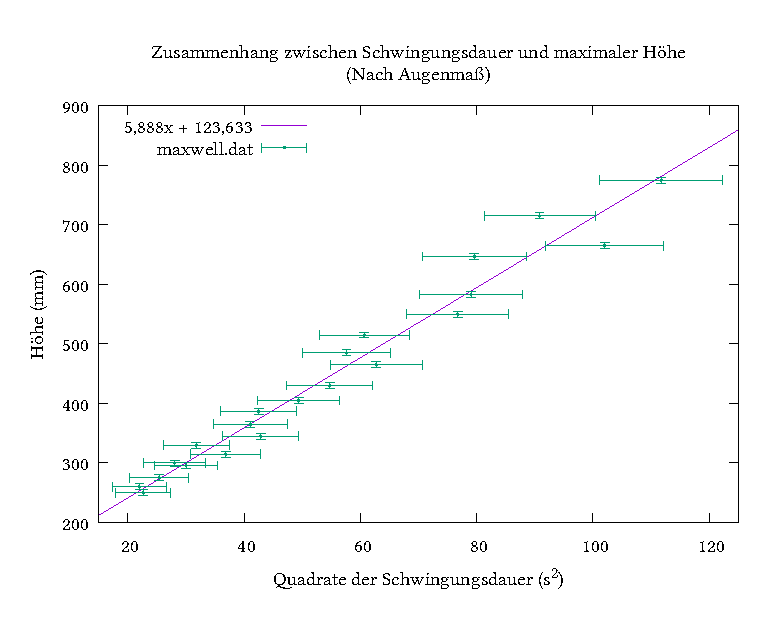
\includegraphics[width=0.9\textwidth]{maxwell.eps}
            \caption{\centering Nach Augenmaß gemessene Werte\hspace{\textwidth}\\$\chi^2_{\text{red}} = 0.343292 < 1 \implies$ Gute Kurvenanpassung\vspace{-1em}}
            \label{fig:stoppuhr}
        \end{figure}
        Wir haben als Endergebnis:
        \begin{center}
            \begin{tabular}{l l}
                \toprule
                $a$ & $\SI{5.8878(2257)}{\milli\meter\per\second\squared}$ \\
                $b$ & $\SI{123.63(1103)}{\milli\meter}$ \\
                \bottomrule
            \end{tabular}
        \end{center}
        \vspace{0.5em}
        Die $y$-Achsenabschnitt $b = \SI{123.63(1103)}{\milli\meter} = \SI{123(12)}{\milli\meter}$ laut der Kurvenanpassung stimmt mit dem gemessenen Wert $h_{0_\text{exp}} = \SI{127(1)}{\milli\meter}$ überein.

        Mit $g = \SI{9.807}{\meter\per\second\squared}$ lässt sich die dimensionslose Größe $y = g/(8a)$ berechnen:
        \begin{equation}
            y = \frac{g}{8a} = \frac{\SI{9.807}{\meter\per\second\squared}}{8 \left(\SI{5,8878e-3}{\meter\per\second\squared}\right)} = \SI{208,2}{} \sigfig{4} \label{eqn:hny}
        \end{equation}

        Aus \eqref{eqn:hn} und \eqref{eqn:hny} folgt auch, dass
        \begin{equation}
            R_{J} = r\sqrt{y-1} = r\sqrt{\frac{g}{8a}-1} = \frac{R_1' + R_1}{2}\sqrt{\frac{g}{8a}-1} \label{eqn:rjorig}
        \end{equation}
        wobei $r = \left(R_1' + R_1\right)/2$ der Wickelradius des Fadens ist.

        \subsubsection{Herleitung des Fehlers mittels Gaußschen-Fehlerfortpflanzung}
            Der Fehler $\Delta R_J$ ist gegeben durch:
            \begin{equation}
                \Delta R_J = \sqrt{\left(\pdv{R_J}{R_1'} \Delta R_1'\right)^2 + \left(\pdv{R_J}{R_1} \Delta R_1\right)^2 + \left(\pdv{R_J}{a} \Delta a\right)^2} \label{eqn:rjfehler}
            \end{equation}
            Die partielle Ableitungen liefern jeweils:
            \begin{align}
                \pdv{R_J}{R_1'} = \pdv{R_J}{R_1} &= \frac{1}{2}\sqrt{\frac{g}{8a} -1} \label{eqn:r1fehler} \\
                \pdv{R_J}{a} &= \frac{1}{2}\left(\frac{R_1' + R_1}{2}\right)\left(\frac{g}{8a} -1\right)^{-\nicefrac{1}{2}}\left(-\frac{g}{8}a^{-2}\right) \notag \\
                &= -\frac{R_1' + R_1}{4\sqrt{\frac{g}{8a} -1}}\cdot \frac{g}{8a^2}
            \end{align}
            Da $\Delta R_1' = \Delta R_1'$, kann man aus \eqref{eqn:r1fehler} die Gleichung \eqref{eqn:rjfehler} vereinfachen:
            \begin{align}
                \Delta R_J &= \sqrt{2\left(\pdv{R_J}{R_1} \Delta R_1\right)^2 + \left(\pdv{R_J}{a} \Delta a\right)^2} \notag \\
                &= \sqrt{2\cdot\frac{1}{4}\left(\frac{g}{8a} -1\right)\left(\Delta R_1\right)^2 + \frac{\left(R_1' + R_1\right)^2}{4\left(\frac{g}{8a} -1\right)}\cdot \frac{g^2}{64a^4}\left(\Delta a\right)^2} \notag \\
                &= \sqrt{\frac{1}{2}\left(\frac{g}{8a} -1\right)\left(\Delta R_1\right)^2 + \frac{g^2\left(R_1' + R_1\right)^2}{32a^3\left(g-8a\right)}\cdot\left(\Delta a\right)^2} \label{eqn:deltarj}
            \end{align}
            
        \subsubsection{Bestimmung von $R_{J}$}
            Mit der folgenden Werten
            \begin{center}
                \begin{tabular}{lrl}
                    \toprule
                    Variable & Wert & Bedeutung \\
                    \midrule
                    $g$ & \SI{9.807}{\meter\per\second\squared} & Erdfeldbeschleunigung \\
                    $R_1$ & \SI{4,05(5)}{\milli\meter} & Radius der Achse \\
                    $R_1'$ & \SI{4,70(5)}{\milli\meter} & Radius der Achse mit Faden \\
                    $a$ & \SI{5.8878(2257)}{\milli\meter\per\second\squared} & Gefundene Steigung der Gerade \\ %\SI{6.517}{\milli\meter\per\second\squared}
                    \bottomrule
                \end{tabular}
            \end{center}

            lässt sich $R_J$ und $\Delta R_J$ bestimmen:
            \begin{align}
                R_{J} &= \frac{R_1' + R_1}{2}\sqrt{\frac{g}{8a}-1} \notag \\
                &= \frac{\SI{4,70}{\milli\meter} + \SI{4,05}{\milli\meter}}{2}\sqrt{\frac{\SI{9.807}{\meter\per\second\squared}}{8\left(\SI{5.8878e-3}{\meter\per\second\squared}\right)}-1} \notag \\
                &= \SI{62,9766}{\milli\meter} \sigfig{6} \\[1em]
                \Delta R_J &= \sqrt{\frac{1}{2}\left(\frac{\SI{9.807}{\meter\per\second\squared}}{8a} -1\right)\left(\Delta R_1\right)^2 + \frac{\left(\SI{9807}{\milli\meter\per\second\squared}\right)^2\left(R_1' + R_1\right)^2}{32a^3\left(\SI{9.807}{\meter\per\second\squared}-8a\right)}\cdot\left(\Delta a\right)^2} \notag \\
                &= \left(\frac{1}{2}\left(\frac{\SI{9807}{\milli\meter\per\second\squared}}{8\left(\SI{5.8878}{\milli\meter\per\second\squared}\right)} -1\right)\left(\SI{0.05}{\milli\meter}\right)^2 \right. \notag \\
                &~~~~+ \left. \frac{\left(\SI{9807}{\milli\meter\per\second\squared}\right)^2\left(\SI{4,70}{\milli\meter} + \SI{4,05}{\milli\meter}\right)^2}{32\left(\SI{5.8878}{\milli\meter\per\second\squared}\right)^3\left(\SI{9807}{\milli\meter\per\second\squared}-8\left(\SI{5.8878}{\milli\meter\per\second\squared}\right)\right)}\cdot\left(\SI{0,2257}{\milli\meter\per\second\squared}\right)^2\right)^{\nicefrac{1}{2}} \notag \\
                &= \SI{2,5}{\milli\meter} \sigfig{2}
            \end{align} % https://tex.stackexchange.com/a/82638
            Daraus folgt: $R_J = \SI{63,0(25)}{\milli\meter}$
    \subsection{Messung mittels gemessener Radien}
        Laut der Anleitung ist der Trägheitsradius $R_J$ gegeben durch:
        \begin{equation}
            R_J = \sqrt{\frac{1}{2}\frac{L_1R_1^4 + L_2\left(R_2^4-R_1^4\right) + L_3\left(R_3^4-R_2^4 + R_5^4-R_4^4\right) + L_4\left(R_4^4-R_3^4\right)}{L_1R_1^2 + L_2\left(R_2^2-R_1^2\right) + L_3\left(R_3^2-R_2^2 + R_5^2-R_4^2\right) + L_4\left(R_4^2-R_3^2\right)}}
        \end{equation}
        mit
        \begin{multicols}{2}
            \begin{center}
                \begin{tabular}{lrl}
                    \toprule
                    Variable & Wert \\
                    \midrule
                    $L_1$ & \SI{141,675(50)}{\milli\meter} \\
                    $L_2$ & \SI{63,275(50)}{\milli\meter} \\
                    $L_3$ & \SI{6.575(50)}{\milli\meter} \\
                    $L_4$ & \SI{2.025(50)}{\milli\meter} \\
                    \bottomrule
                \end{tabular}
            \end{center}
            \begin{center}
                \begin{tabular}{lrl}
                    \toprule
                    Variable & Wert \\
                    \midrule
                    $R_1$ & \SI{4,05(5)}{\milli\meter} \\
                    $R_2$ & \SI{6.525(50)}{\milli\meter} \\
                    $R_3$ & \SI{10.25(5)}{\milli\meter} \\
                    $R_4$ & \SI{67.85(5)}{\milli\meter} \\
                    $R_5$ & \SI{87.05(5)}{\milli\meter} \\
                    \bottomrule
                \end{tabular}
            \end{center}
        \end{multicols}
        
        Die Werte bzw. Messunsicherheiten wurden an dieser Stelle nicht gerundet, da es sich um Zwischenergebnissen handelt. Die Einheiten wurden beim Einsetzen auch nur am Ende berücksichtigt.

        \begin{minipage}[t][2cm][t]{1.1\textwidth}
            \tiny
            \vspace{-2em}
            \begin{align*}
                R_J &= \sqrt{\frac{1}{2}\frac{L_1R_1^4 + L_2\left(R_2^4-R_1^4\right) + L_3\left(R_3^4-R_2^4 + R_5^4-R_4^4\right) + L_4\left(R_4^4-R_3^4\right)}{L_1R_1^2 + L_2\left(R_2^2-R_1^2\right) + L_3\left(R_3^2-R_2^2 + R_5^2-R_4^2\right) + L_4\left(R_4^2-R_3^2\right)}} \\
                &= \left(\frac{1}{2}\frac{\left(\SI{141,675}{}\right)\left(\SI{4.05}{}\right)^4 + \left(\SI{63.275}{}\right)\left(\left(\SI{6.525}{}\right)^4-\left(\SI{4.05}{}\right)^4\right) + \left(\SI{6.575}{}\right)\left(\left(\SI{10.25}{}\right)^4-\left(\SI{6.525}{}\right)^4 + \left(\SI{87.05}{}\right)^4-\left(\SI{67.85}{}\right)^4\right) + \left(\SI{2.025}{}\right)\left(\left(\SI{67.85}{}\right)^4-\left(\SI{10.25}{}\right)^4\right)}{\left(\SI{141,675}{}\right)\left(\SI{4.05}{}\right)^2 + \left(\SI{63.275}{}\right)\left(\left(\SI{6.525}{}\right)^2-\left(\SI{4.05}{}\right)^2\right) + \left(\SI{6.575}{}\right)\left(\left(\SI{10.25}{}\right)^2-\left(\SI{6.525}{}\right)^2 + \left(\SI{87.05}{}\right)^2-\left(\SI{67.85}{}\right)^2\right) + \left(\SI{2.025}{}\right)\left(\left(\SI{67.85}{}\right)^2-\left(\SI{10.25}{}\right)^2\right)}\right)^{\nicefrac{1}{2}}
            \end{align*}
        \end{minipage}

        Nach sorgfältiger Rechnung erhalten wir $R_J = \SI{65.2296}{\milli\meter} = \SI{65.2}{\milli\meter} \sigfig{3}$.

        Da die Gleichung zu kompliziert ist. wurde eine (etwas inelegante) \texttt{Python} Skript durchgeführt, um die minimale bzw. maximale Werte von $R_J$ zu schätzen (Siehe Appendix \ref{appdx:pythonTV2}). Die echte minimale und maximale Werte von $R_J$ wurden dann mithilfe eines Taschenrechners bestimmt:
        \begin{center}
            \begin{tabular}{l ll r}
                \toprule
                $R_J$ & Var muss maximal sein & Var muss minimal sein & Wert \\
                \midrule
                Max & $L_3$, $R_5$ & $L_1$, $L_2$, $L_4$, $R_1$, $R_2$, $R_3$, $R_4$ & $\SI{65.5096}{\milli\meter}$\\
                Min & $L_1$, $L_2$, $L_4$, $R_1$, $R_2$, $R_3$, $R_4$ & $L_3$, $R_5$ & $\SI{64.9498}{\milli\meter}$\\
                \bottomrule
            \end{tabular}
        \end{center}
        Da die obere und untere Grenze symmetrisch ist, ist der Fehler dann $\left(\maxi{R_J} - \mini{R_J}\right)/2 = \SI{0.28}{\milli\meter}$.

        Daraus folgt, dass $R_J = \SI{65.23(28)}{\milli\meter}$.

    \subsection{Diskussion 1}
        \begin{center}
            \begin{tabular} {lr}
                \toprule
                $R_J$ & Wert \\
                \midrule
                Augenmaß & \SI{63,0(25)}{\milli\meter} \\
                Radienmessung & \SI{65.23(28)}{\milli\meter} \\
                \bottomrule
            \end{tabular}
        \end{center}

        % Obwohl der durch Radienmessung bestimmte Wert $R_{J_r}$ nicht im Fehlerintervall des durch Augenmaß bestimmten Wert $R_{J_a}$ liegt, liegt es innerhalb im dreifachen des Fehlerintervalls. Das Ergebnis $R_{J_a}$ ist deshalb verträglich mit dem Vergleichswert $R_{J_r}$. 

        Der durch Radienmessung bestimmte Wert $R_{J_r}$ liegt im Fehlerintervall des durch Augenmaß bestimmten Wert $R_{J_a}$. Das Ergebnis $R_{J_a}$ stimmt mit dem Vergleichswert $R_{J_r}$ überein. 

        Der Fehler $\Delta R_{J_a}$ ist aber deutlich größer als den Fehler $\Delta R_{J_r}$. Dieser Unterschied kann zu der Ungenauigkeit der Messmethode und der Schwankungen des Rads während der Auf- und Abrollens zurückgeführt. Wie im ersten Abschnitt schon erwähnt hat, war es auch schwer den Umkehrpunkt mit Augenmaß genau zu bestimmen. 

        Beide Methode haben ihren eigenen Vorteil. Augenmaß ist eher ungenau und zeitintensiv, aber führt zu einer einfacheren Rechnung. Stattdessen ist die Radienmessung genauer, aber führt zu Schwierigkeiten bei der Fehlerbestimmung. 

    \subsection{Messung mittels Ultraschall-Bewegungssensor}
        Aus dem Protokoll sind unsere Erwartungen wie folgt:
        \begin{center}
            \begin{tabular}{l p{0.7\textwidth}}
                \toprule
                Höhe & Aneinandergereihte, nach unten geöffnete Parabelbögen mit abnehmende Höhe \\
                Geschwindigkeit & "Sägezahnkurve", also linear steigende Geschwindigkeit mit Sprüngen zwischen den Perioden von minimaler zu maximaler Geschwindigkeit. \\
                Beschleunigung & Konstante Beschleunigung $< g$; an Umkehrpunkten sehr hohe Beschleunigung. \\
                \bottomrule
            \end{tabular}
        \end{center}

        Unsere Erwartungen stimmen mit den Diagrammen aus \textit{LoggerPro} großenteils überein, besonders bei der Position-Zeit Diagramme. Die größte Abweichungen lässt sich im Beschleunigung-Zeit Diagramme erfahren. Zwischen den Peaks sollte die Beschleunigung theoretisch konstant bleiben, aber es gibt im diesen Fall große Abweichungen im Form von Geräusch. 

        Das kann vermutlich auf die Art und Weise zurückführen, wie \textit{LoggerPro} diese Diagramme erzeugt hat. Zwischen jeder zwei nacheinander folgender Positionspunkte würden wahrscheinlich die Differenz und "Steigung" gerechnet und dann geplottet. Die Beschleunigung könnte auch so von Geschwindigkeitspunkten berechnet werden. Das könnte zu der Situation führen, indem kleine Abweichungen bzw. Geräusche bei den Positionspunkten mit der Rechnung der Geschwindigkeitspunkten vergrößert würden. Diese Vergrößerung verstärkt sich weiter mit der Rechnung der Beschleunigung. Deswegen entstehen in den Diagramme die Abweichungen von unserer Erwartungen.

        Der von Computer berechnete $y$-Achsenabschnitt liegt bei $\SI{-0.0167(21)}{\meter} = \SI{-1.67(21)}{\centi\meter}$, was der Nullpunkt ziemlich nah liegt. Der Nullpunkt liegt trotzdem nicht in dem Fehlerintervall dieses Wertes. Manuelles Nachmessen ergab jedoch, dass sich die Höhe des Rades während dem Versuch nicht geändert hat. Der Fehler könnte bei der manuellen Auswahl der Umkehrpunkte im Diagramm entstanden sein. 

        \subsubsection{Bestimmung von $R_J$}
            Die Rechnung erfolgt wie vorher. Mit der folgenden Werten
            \begin{center}
                \begin{tabular}{lrl}
                    \toprule
                    Variable & Wert & Bedeutung \\
                    \midrule
                    $g$ & \SI{9.807}{\meter\per\second\squared} & Erdfeldbeschleunigung \\
                    $R_1$ & \SI{4,05(5)}{\milli\meter} & Radius der Achse \\
                    $R_1'$ & \SI{4,70(5)}{\milli\meter} & Radius der Achse mit Faden \\
                    $a$ & \SI{5.69714(3033)}{\milli\meter\per\second\squared} & Erhaltene Steigung (Ultraschall-Sensor) \\ %\SI{6.517}{\milli\meter\per\second\squared}
                    \bottomrule
                \end{tabular}
            \end{center}

            lässt sich $R_J$ und $\Delta R_J$ mithilfe \eqref{eqn:rjorig} und \eqref{eqn:deltarj} bestimmen:
            \begin{align}
                R_{J} &= \frac{R_1' + R_1}{2}\sqrt{\frac{g}{8a}-1} \notag \\
                &= \frac{\SI{4,70}{\milli\meter} + \SI{4,05}{\milli\meter}}{2}\sqrt{\frac{\SI{9.807}{\meter\per\second\squared}}{8\left(\SI{5.69714e-3}{\meter\per\second\squared}\right)}-1} \notag \\
                &= \SI{64.0267}{\milli\meter} \sigfig{6} \\[1em]
                \Delta R_J &= \sqrt{\frac{1}{2}\left(\frac{\SI{9.807}{\meter\per\second\squared}}{8a} -1\right)\left(\Delta R_1\right)^2 + \frac{\left(\SI{9807}{\milli\meter\per\second\squared}\right)^2\left(R_1' + R_1\right)^2}{32a^3\left(\SI{9.807}{\meter\per\second\squared}-8a\right)}\cdot\left(\Delta a\right)^2} \notag \\
                &= \left(\frac{1}{2}\left(\frac{\SI{9807}{\milli\meter\per\second\squared}}{8\left(\SI{5.69714}{\milli\meter\per\second\squared}\right)} -1\right)\left(\SI{0.05}{\milli\meter}\right)^2 \right. \notag \\
                &~~~~+ \left. \frac{\left(\SI{9807}{\milli\meter\per\second\squared}\right)^2\left(\SI{4,70}{\milli\meter} + \SI{4,05}{\milli\meter}\right)^2}{32\left(\SI{5.69714}{\milli\meter\per\second\squared}\right)^3\left(\SI{9807}{\milli\meter\per\second\squared}-8\left(\SI{5.69714}{\milli\meter\per\second\squared}\right)\right)}\cdot\left(\SI{0,03033}{\milli\meter\per\second\squared}\right)^2\right)^{\nicefrac{1}{2}} \notag \\
                &= \SI{0.7}{\milli\meter} \sigfig{1}
            \end{align} % https://tex.stackexchange.com/a/82638
            Daraus folgt: $R_J = \SI{64.0(7)}{\milli\meter}$

    \newpage
    \subsection{Diskussion 2}
        \begin{center}
            \begin{tabular} {lr}
                \toprule
                $R_J$ & Wert \\
                \midrule
                Augenmaß & \SI{63,0(25)}{\milli\meter} \\
                Radienmessung & \SI{65.23(28)}{\milli\meter} \\
                Ultraschall-Sensor & \SI{64.0(7)}{\milli\meter} \\
                \bottomrule
            \end{tabular}
        \end{center}

        Die Fehlerintervalle der manuellen durch Augenmaß bestimmte Messung und der computergestützten Messung überschneiden sich auch wie bei der Radienmessung. Die Werte stimmen in Rahmen der Messgenauigkeit überein. 

        Der durch Radienmessung erhaltene Wert von $R_J$ liegt nur in dreifachen des Fehlerintervalls des computergestützten Wertes. Die Werte sind also verträglich miteinander. Dieser Unterschied ist vermutlich dadurch entsteht, dass die Ungenauigkeit der Ultraschall-Sensor bezüglich zeitlicher und örtlicher Messungen nicht berücksichtigt wurde.

        Der Schwerpunkt eines Körpers gibt an, wo sich ein Massenpunkt gleicher Masse in einem konservative Gravitationskraftfeld befinden müsste, um die gleiche Beschleunigung zu erfahren. Analog dazu gibt der Trägheitsradius an, wo sich ein Massenpunkt gleicher Masse befinden müsste, um das gleiche Drehmoment mit einer bestimmter Kraft um einer bestimmter Rotationsachse zu erfahren.